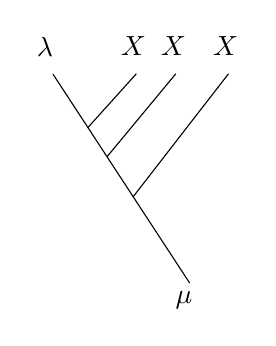
\begin{tikzpicture}[yscale=-1,scale=0.015,baseline={([yshift=-.5ex]current bounding box.center)}]
\begin{scope}[shift={(0.00mm,719.29mm)}]
% path id='path4136'
% path spec='M 148.57143,-716.2092 1305.7143,1052.3623'
\draw [fill=none,draw=black] (148.57mm,-716.21mm)
-- (1305.71mm,1052.36mm)
;
% path id='path4138'
% path spec='M 444.46712,-263.86654 854.65033,-719.23876'
\draw [fill=none,draw=black] (444.47mm,-263.87mm)
-- (854.65mm,-719.24mm)
;
% path id='path4140'
% path spec='M 606.16072,-16.477057 1188.8393,-719.24492'
\draw [fill=none,draw=black] (606.16mm,-16.48mm)
-- (1188.84mm,-719.24mm)
;
% path id='path4142'
% path spec='M 827.72322,321.87112 1634.7768,-719.11098'
\draw [fill=none,draw=black] (827.72mm,321.87mm)
-- (1634.78mm,-719.11mm)
;
\node [black] at (80.84mm,-950mm) { $\lambda$ };
\node [black] at (829.21mm,-950mm) { $X$ };
\node [black] at (1168.47mm,-950mm) { $X$ };
\node [black] at (1610.14mm,-950mm) { $X$ };
\node [black] at (1258.65mm,1200mm) { $\mu$ };
\end{scope}
\end{tikzpicture}
